
\section{SeVN Problem Formulation}
\label{sec:ProblemFormulation}

\cite{cui2016big}
In this section, From above section Sec.\ref{sec:Introduction}, we extract problem definition of the SeVN problem as follows: for a given VN request which had been embedded into SN with N task nodes, then survive the eVN with
some additional nodes , a set of appropriate links to connect these N+k nodes and match node's function type, and reserve sufficient computing/communication resources in these nodes/links to guarantee the restorability of eVN request after a facility node failure.

For simplicity, we firstly introduce some notations and definitions about graph's fault tolerant in order to describe our proposed SeVN problem clearly.

\subsection{Node Fault Graph}
\subsubsection{Node Fault tolerant (NFT)}
We refer to the concept of $k$-NFT\cite{harary1996node}. Let $G(V,E)$ be a graph with $n$ nodes and $q$ edges. An $(n+k)$-node graph $G^*$ is k-node fault-tolerant, or $k$-NFT, with respect to $G$ if every graph $G^*-R$ obtained by removing any nodes set $R$ of $k>0$ nodes from $G^*$ contains $G$. Generally speaking, $G$ is subgraph isomorphism of $G^*-R$. We will refer to $G^*$ as a $k$-NFT supergraphs of $G$ or simply as a $k$-NFT($G$). We also say $G^*\cong$ $k$-NFT($G$), the set of all k-NFT($G$) supergraphs of $G$.

The complete graph $K_{n+k}$ of $n + k$ nodes is trivially a k-NFT supergraph of every $G$ that contains up to n nodes. We are concerned mainly with $k$-NFT graphs that satisfy the following optimality criterion: If $G^*$ has the smallest number $|E(G^*)|$ of edges among all $(n + k)$-node supergraphs that are $k$-NFT with respect to $G$, then $G^*$ is optimally $k$-NFT with respect to $G$. The number $NFT_{ec}$$(G,k)$ =$|E(G^*)-E(G)|$ is called the $k$-NFT edge cost of $G$. The number $NFT_{nc}$$(G,k)$ =$|V(G^*)-V(G)|$ is called the $k$-NFT node cost of $G$, however $NFT_{nc}$$(G,k)$ = k with respect with k node fault tolerant graph of graph $G$ . For example, $NFT_{nc}$$(C_5,1)$ and $NFT_{ec}$$(C_5,1)$ of graph $C_5$ is 1 and 5 respectively as demonstrated in Fig.\ref{fig:NFTexample}. Furthermore, deriving optimal graphs $G^o$ with minimal links for any general graph G has exponential complexity. To the best of the authors’ knowledge, optimal solutions are found only on regular graphs such as lines, square-grids, circles, and trees.

\begin{figure}
  \centering
  % Requires \usepackage{graphicx}
  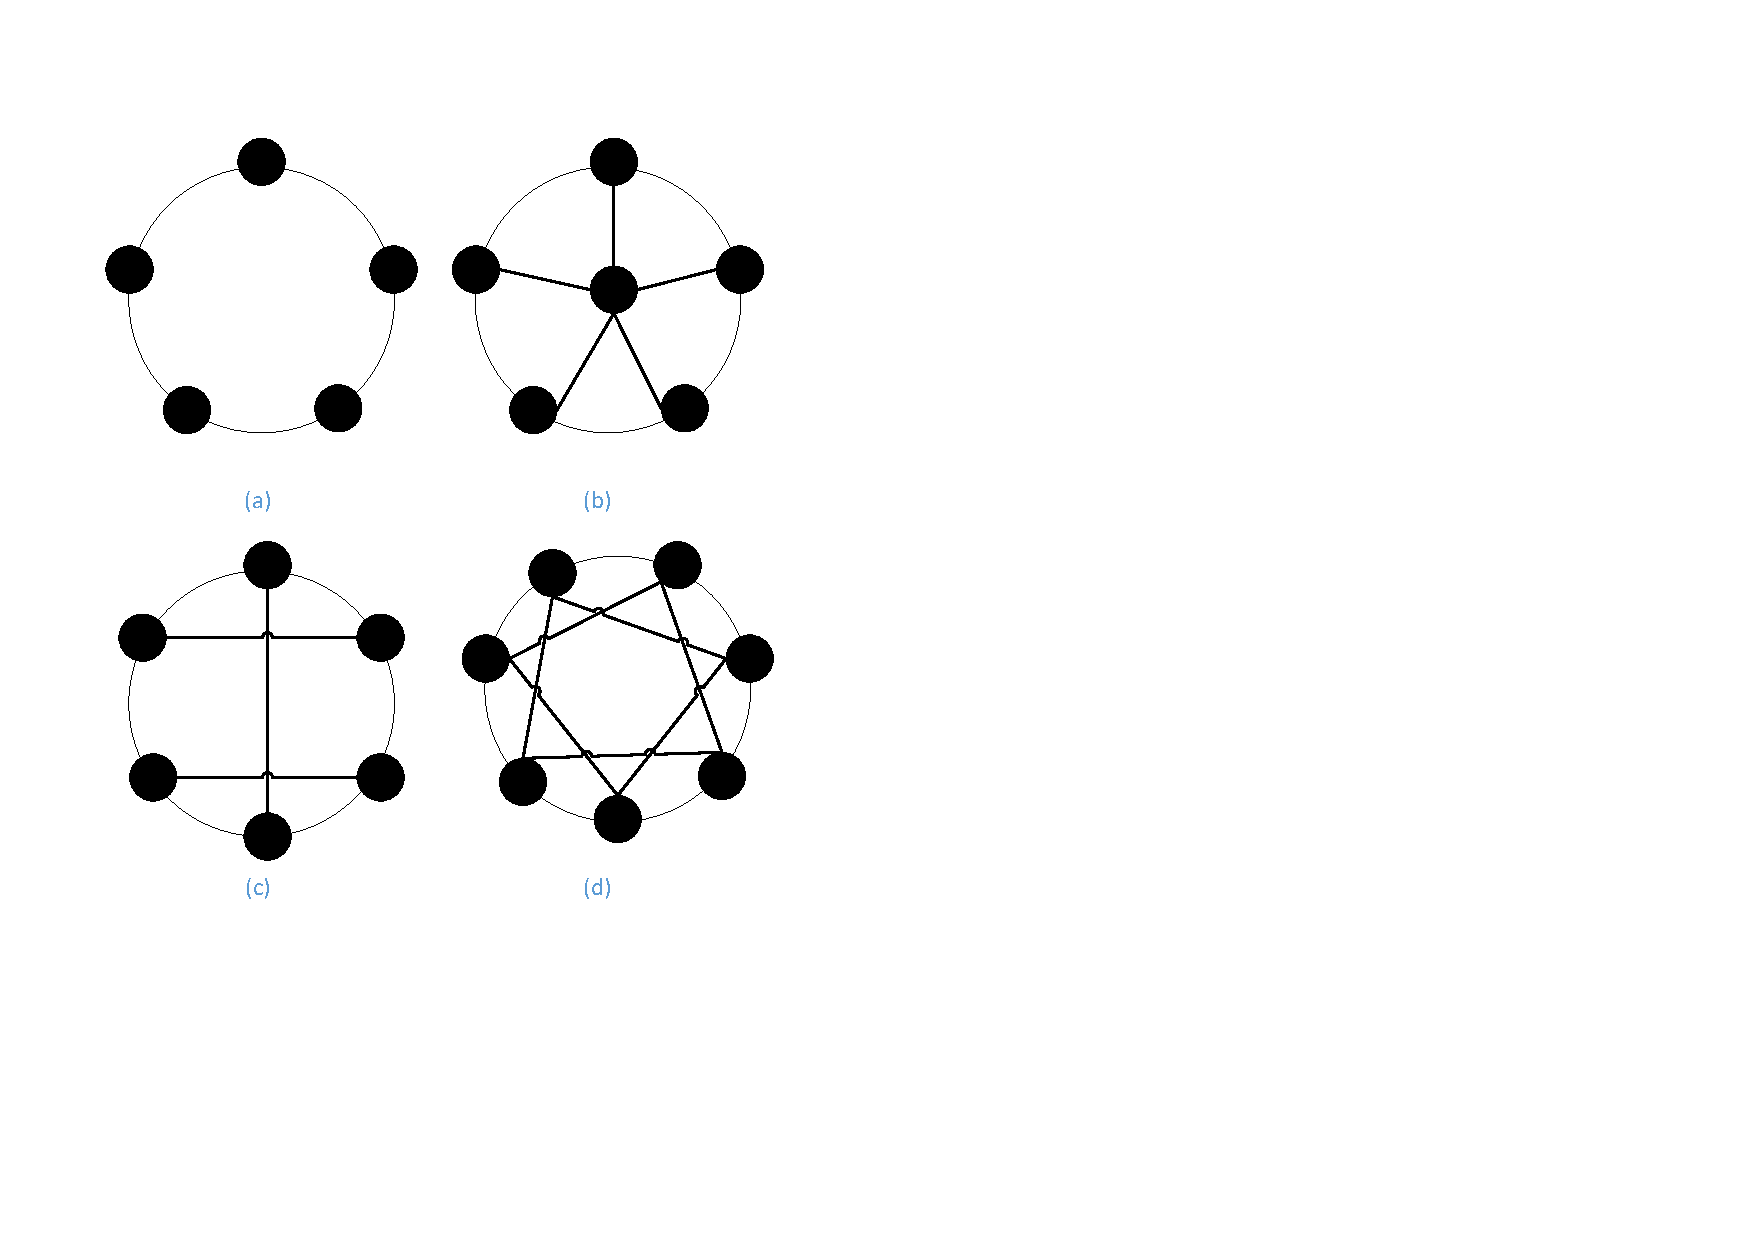
\includegraphics[width=2.5in]{Fig/NFTexample}\\
  \caption{(a)The cycle $C_5$; (b)a nonoptimal $1$-NFT($C_5$), $|R|$=1 ; (c) an optimal $1$-NFT($C_5$), $|R|$=1; (d) an optimal $2$-NFT($C_5$), $|R|$=2. }\label{fig:NFTexample}
\end{figure}

\subsubsection{Function Node Fault Tolerant (FNFT)}
When every nodes of graph $G(V,E,S)$ have a specific functions set $S$ (corresponding to node's function function set) and every nodes is marked by only one function type (every node of virtual network just run only one type of function function), which is denoted by node function. A $(n+k)$-node graph $G^o$ is k-function node fault tolerant, or $k$-FNFT, with respect to $G(V,E,S)$ if every graph $G^o-R$ obtained by removing any nodes set $R$ of $k>0$ nodes from $G^o$ contains $G$, $G$ is subgraph isomorphism of $G^o-R$ and the node function of any nodes $n$ of $G$ belong function set of node $n^o$ corresponding to node $n$. We will refer to $G^o$ as a $k$-FNFT supergraphs of $G$ or simply as a $k$-FNFT($G$). The number $SNFT_{nc}$$(G,k)$ =$|V(G^o)-V(G)|$ is called the $k$-FNFT node cost of $G$. The number $SNFT_{ec}$$(G,k)$ =$|E(G^o)-E(G)|$ is called the $k$-FNFT edge cost of $G$. Suppose every node of added nodes contain all function types in current above definition.
\subsubsection{FNFT with B}
After our simple inference, if we refer the node cost $FNFT_{nc}(G,k)$  is more important cost than $FNFT_{ec}(G,k)$  edge cost, moreover the added node $B(V,S)$ could have a function set rather than contain all types of function (every node of substrate network contain various combinations of function type), Based real situation that the added node should be limited in specific function set through our analyzing the real-world practical phenomenon.(should cite a paper).
 As shown in Fig
%A backup (redundant) node b must not be able to assume full execution of a failed critical node c.

Suppose added nodes as backup node set $B(V,S)$, where every nodes of backup node set $B$ have a function set. The $k$-FNFT($G,B$) is denoted by requesting a k function node fault tolerant graph of graph $G$ and added nodes belong backup nodes set $B$. For example, as shown in Fig.\ref{fig:SNFTBexample}, every backup node have individual function set. In Fig.\ref{fig:SNFToptimal_n1Fail} displaying the transformed graph after node $v_1$ failure.

%The limited node of $G^o-G$ with respect to any $G^o$ is used as inserted node from specific node set $B$ which is premise. k-specific node fault-tolerant graph of $G$ with limit-inserted node set $B$ is denoted by k-FNFT($G,B$).


\begin{figure*}[tp]
\centering
\begin{minipage}[t]{0.3\linewidth}
\centering
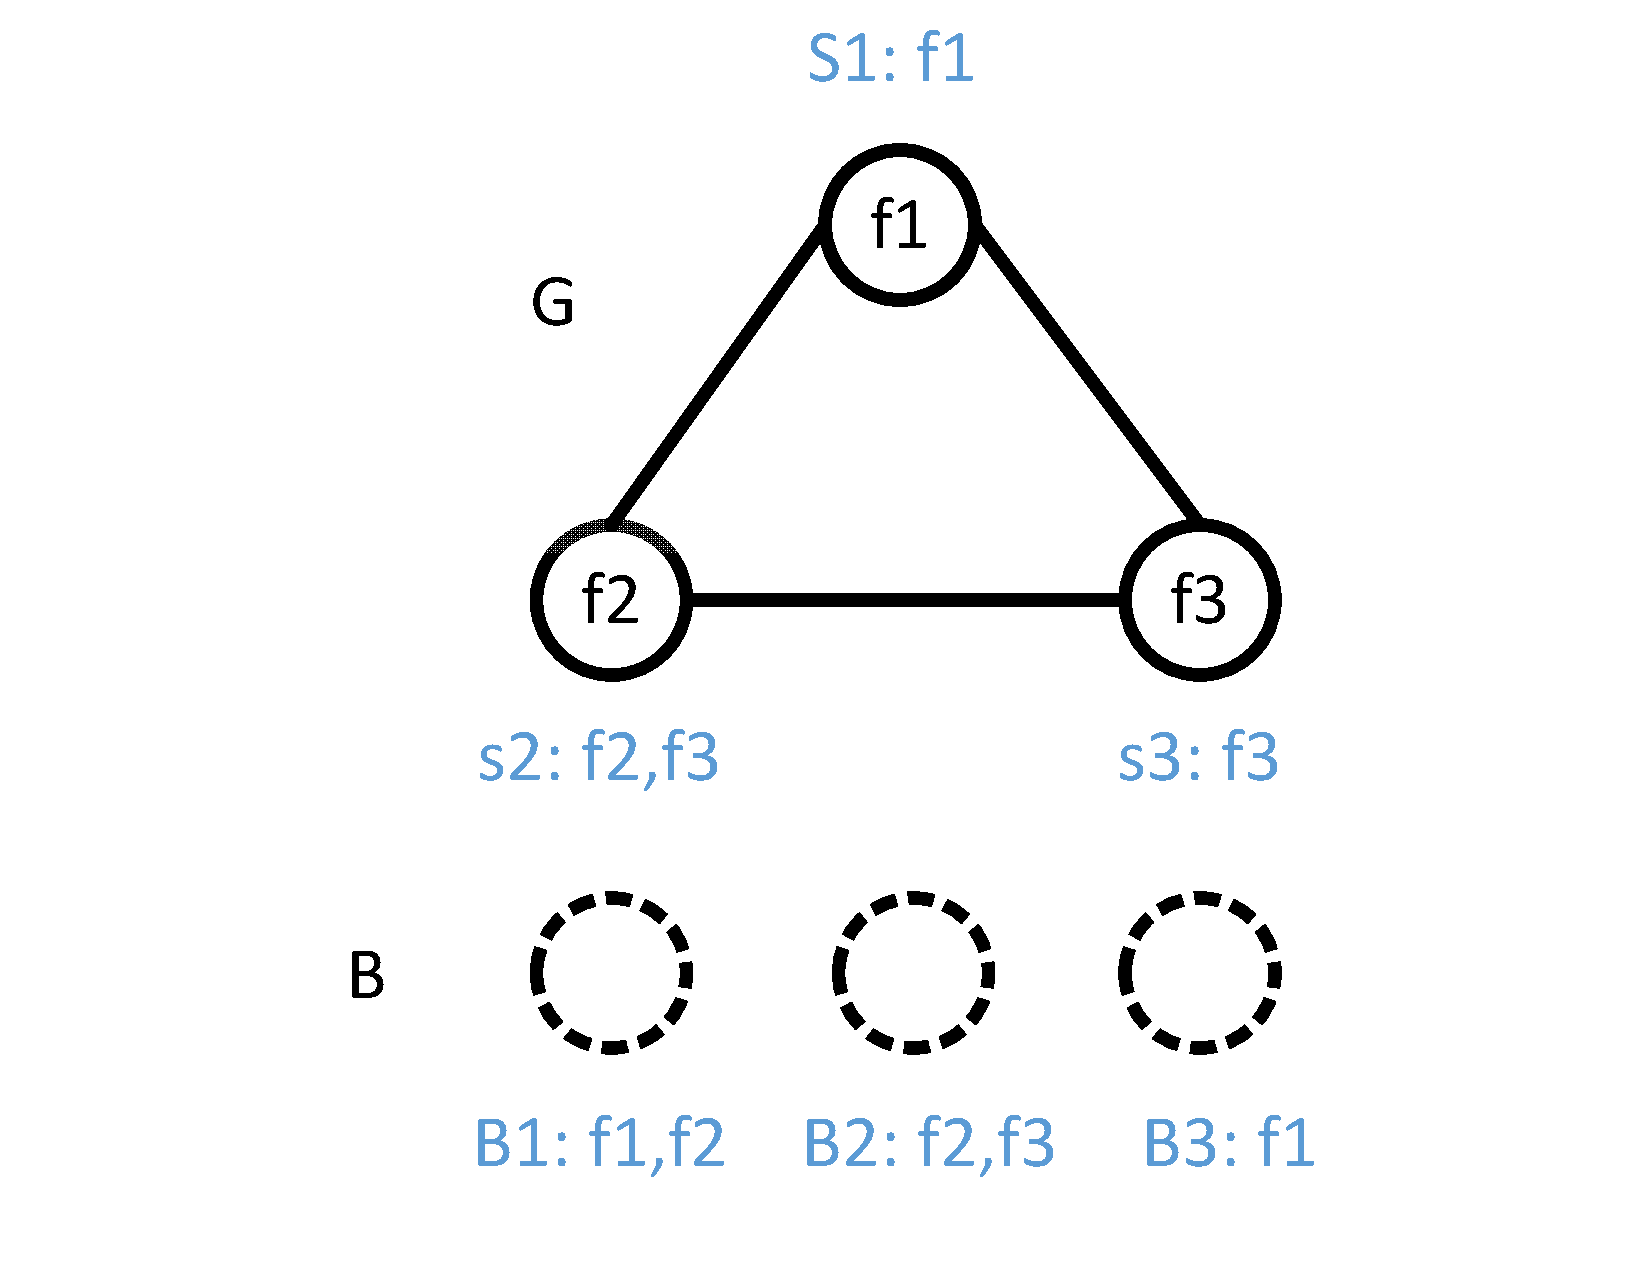
\includegraphics[width=1.5in]{Fig/SNFTBexample}\\
\caption{Graph $G(V,E,S)$: V=$\{v_1,v_2,v_3\}$, E=$\{v_1v_2,v_2v_3,v_3v_1\}$, S=$\{\{s_1\},\{s_2,s_3\},\{s_3\}\}$. Backup node $B(V,S)$: V=$\{b_1,b_2,b_3\}$, S=$\{\{s_1,s_2\},\{s_2,s_3\},\{s_1\}\}$ }\label{fig:SNFTBexample}
\end{minipage}
\hfill
\begin{minipage}[t]{0.3\linewidth}
\centering
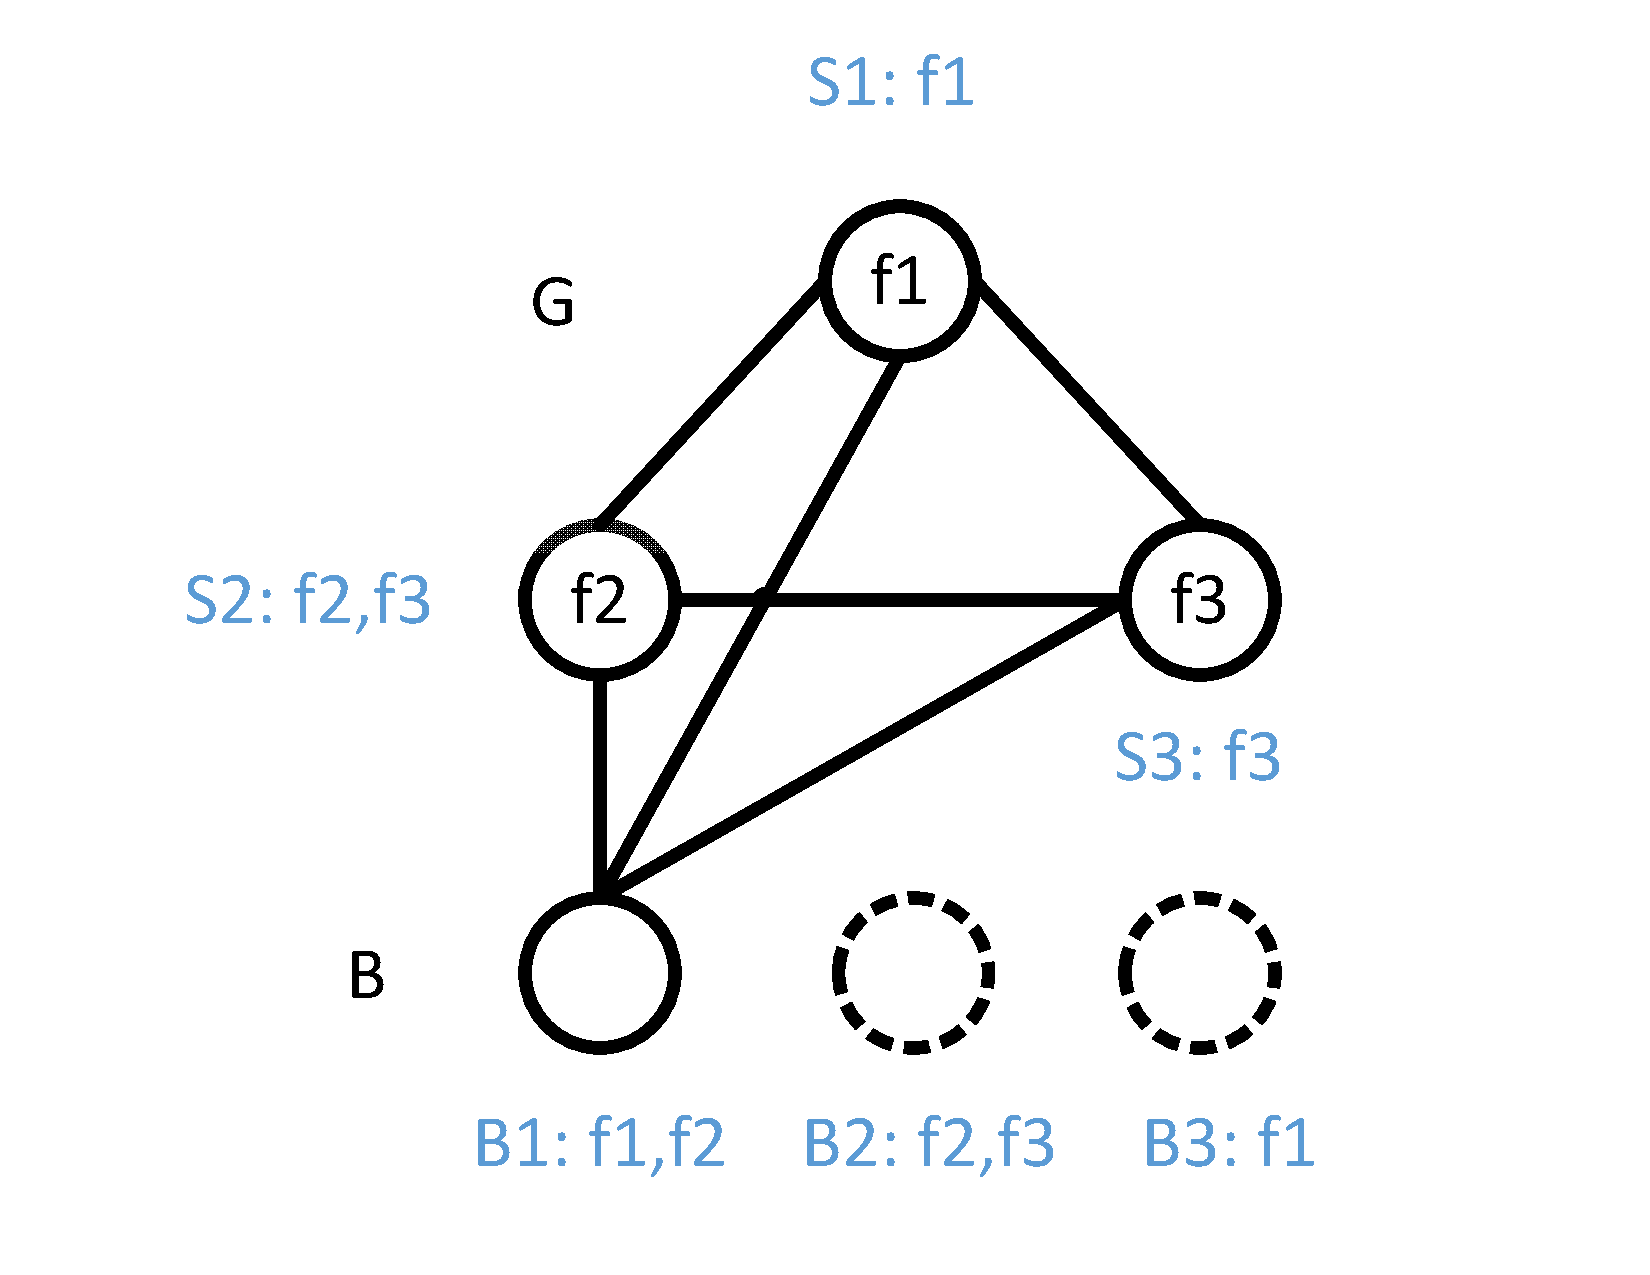
\includegraphics[width=1.5in]{Fig/SNFToptimal}\\
\caption{optimal $1$-FNFT($G(V,E,S),B(V,S)$), $SNFT_{nc}$$(G,1,B)$=1, $SNFT_{ec}$$(G,1,B)$=3.}\label{fig:SNFToptimal}
\end{minipage}
\hfill
\begin{minipage}[t]{0.3\linewidth}
\centering
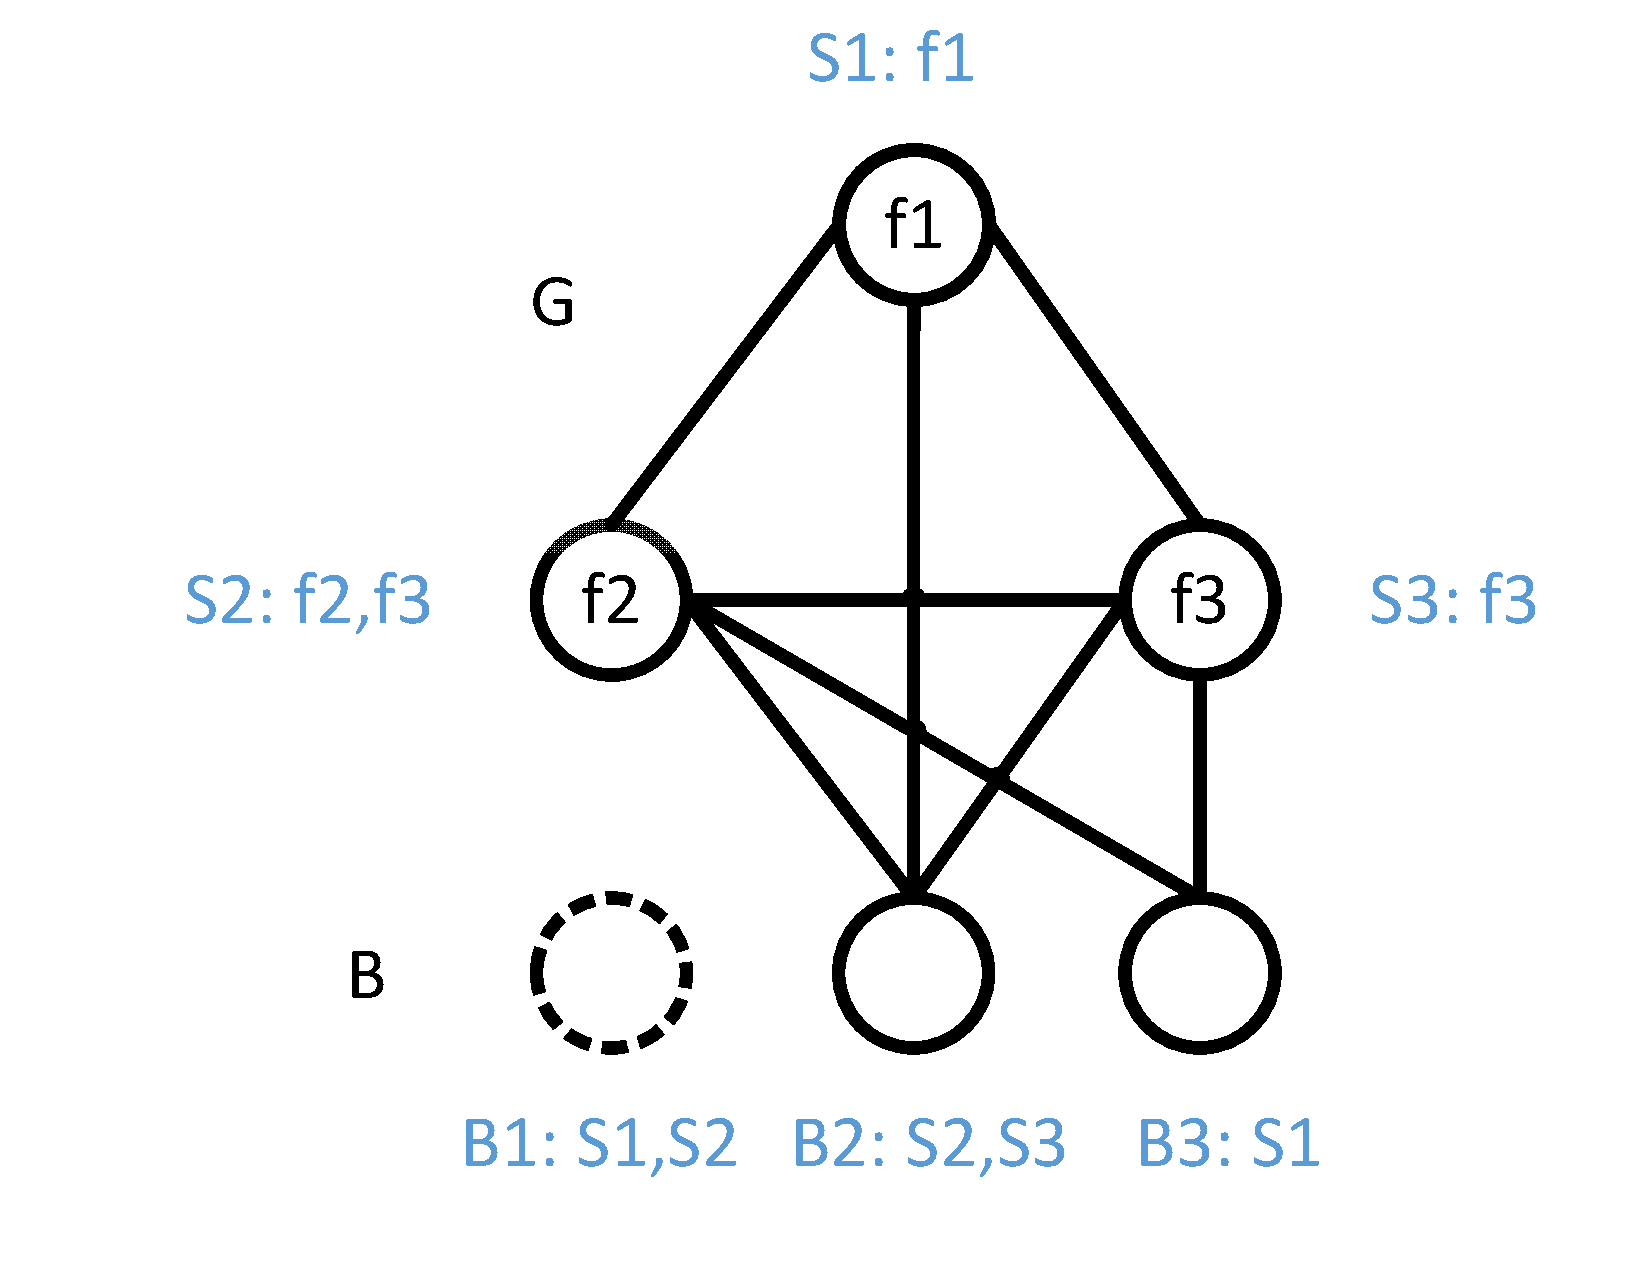
\includegraphics[width=1.5in]{Fig/SNFTnonoptimal}\\
\caption{non optimal $k$-FNFT($G(V,E,S),B(V,S)$), $SNFT_{nc}$$(G,1,B)$=2, $SNFT_{ec}$$(G,1,B)$=5}\label{fig:SNFTnonoptimal}
\end{minipage}
\end{figure*}


\begin{figure*}[tp]
\centering
\begin{minipage}[t]{0.3\linewidth}
\centering
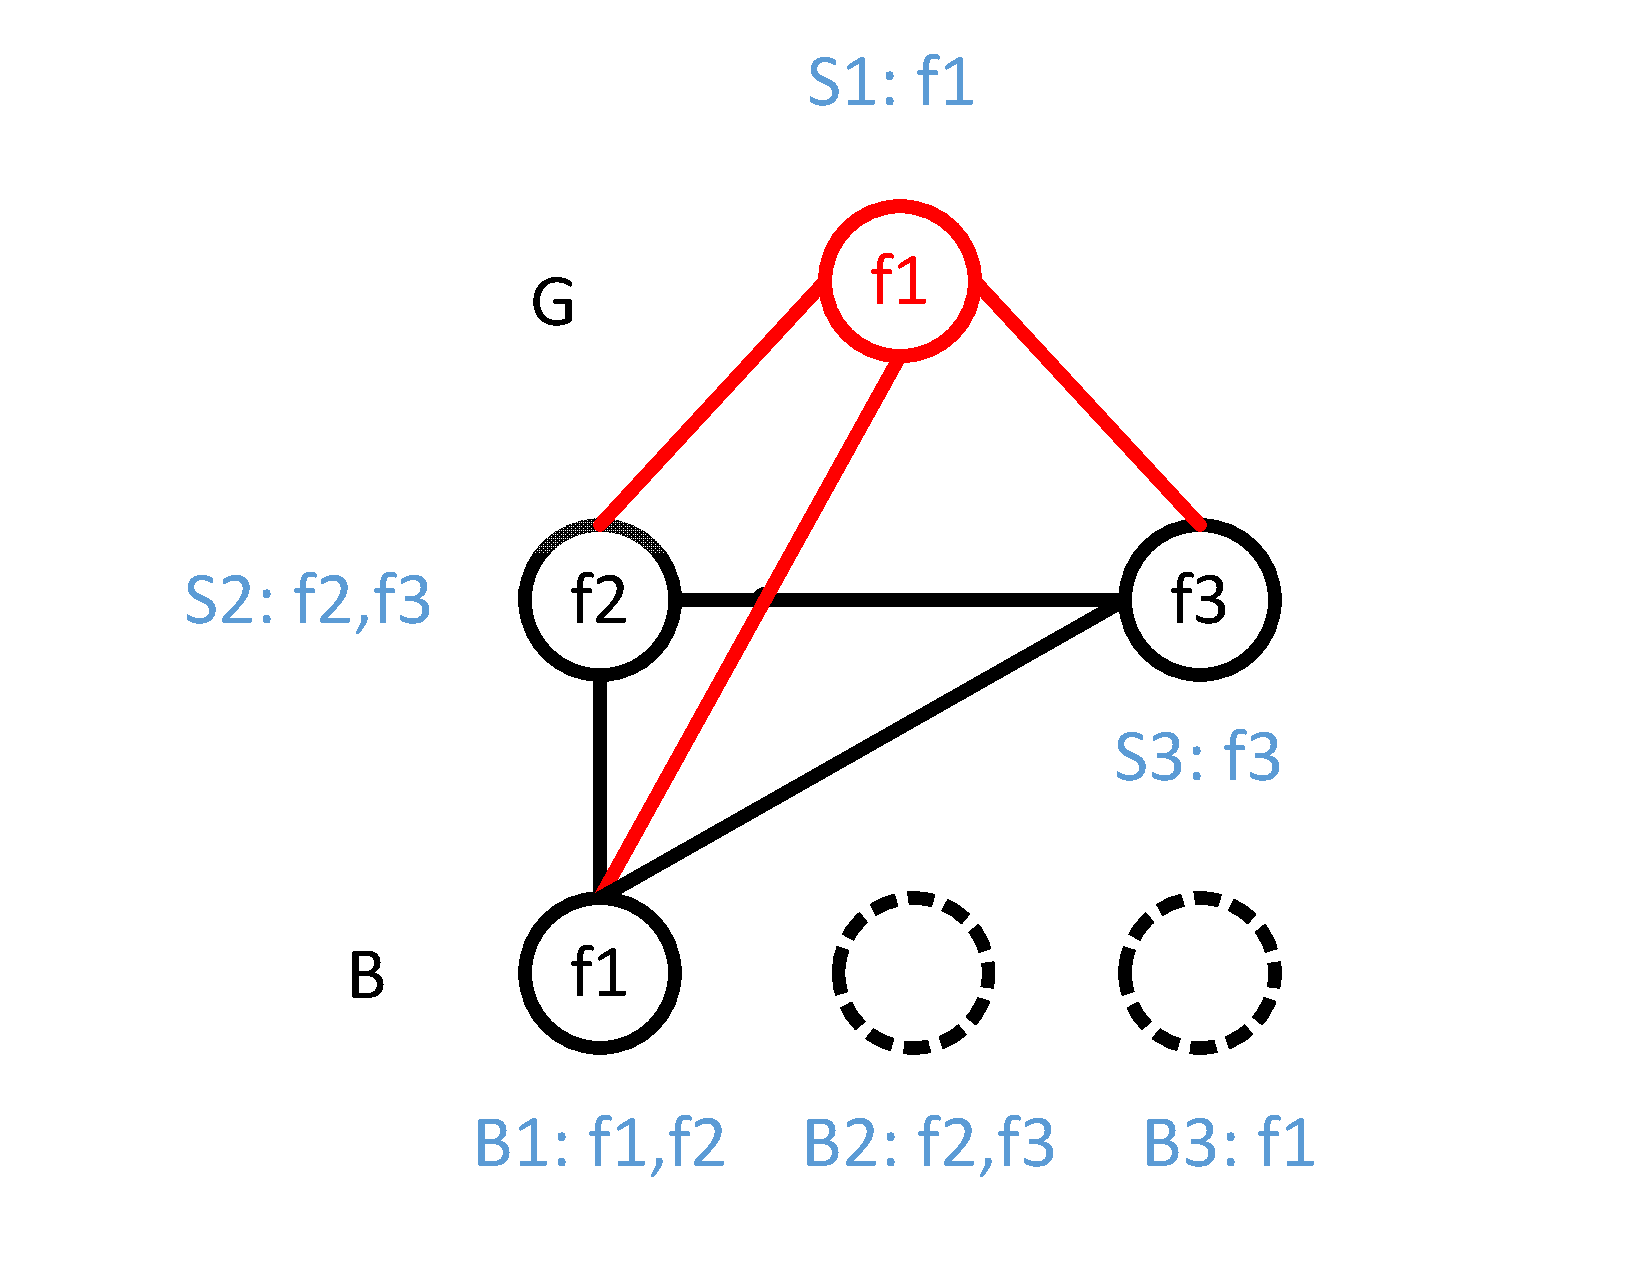
\includegraphics[width=1.5in]{Fig/SNFToptimal_n1Fail}\\
\caption{optimal $k$-FNFT($G(V,E,S),B(V,S)$) when node $v_1$ fail, node $v_1$ transform to $b_1$}\label{fig:SNFToptimal_n1Fail}
\end{minipage}
\hfill
\begin{minipage}[t]{0.3\linewidth}
\centering
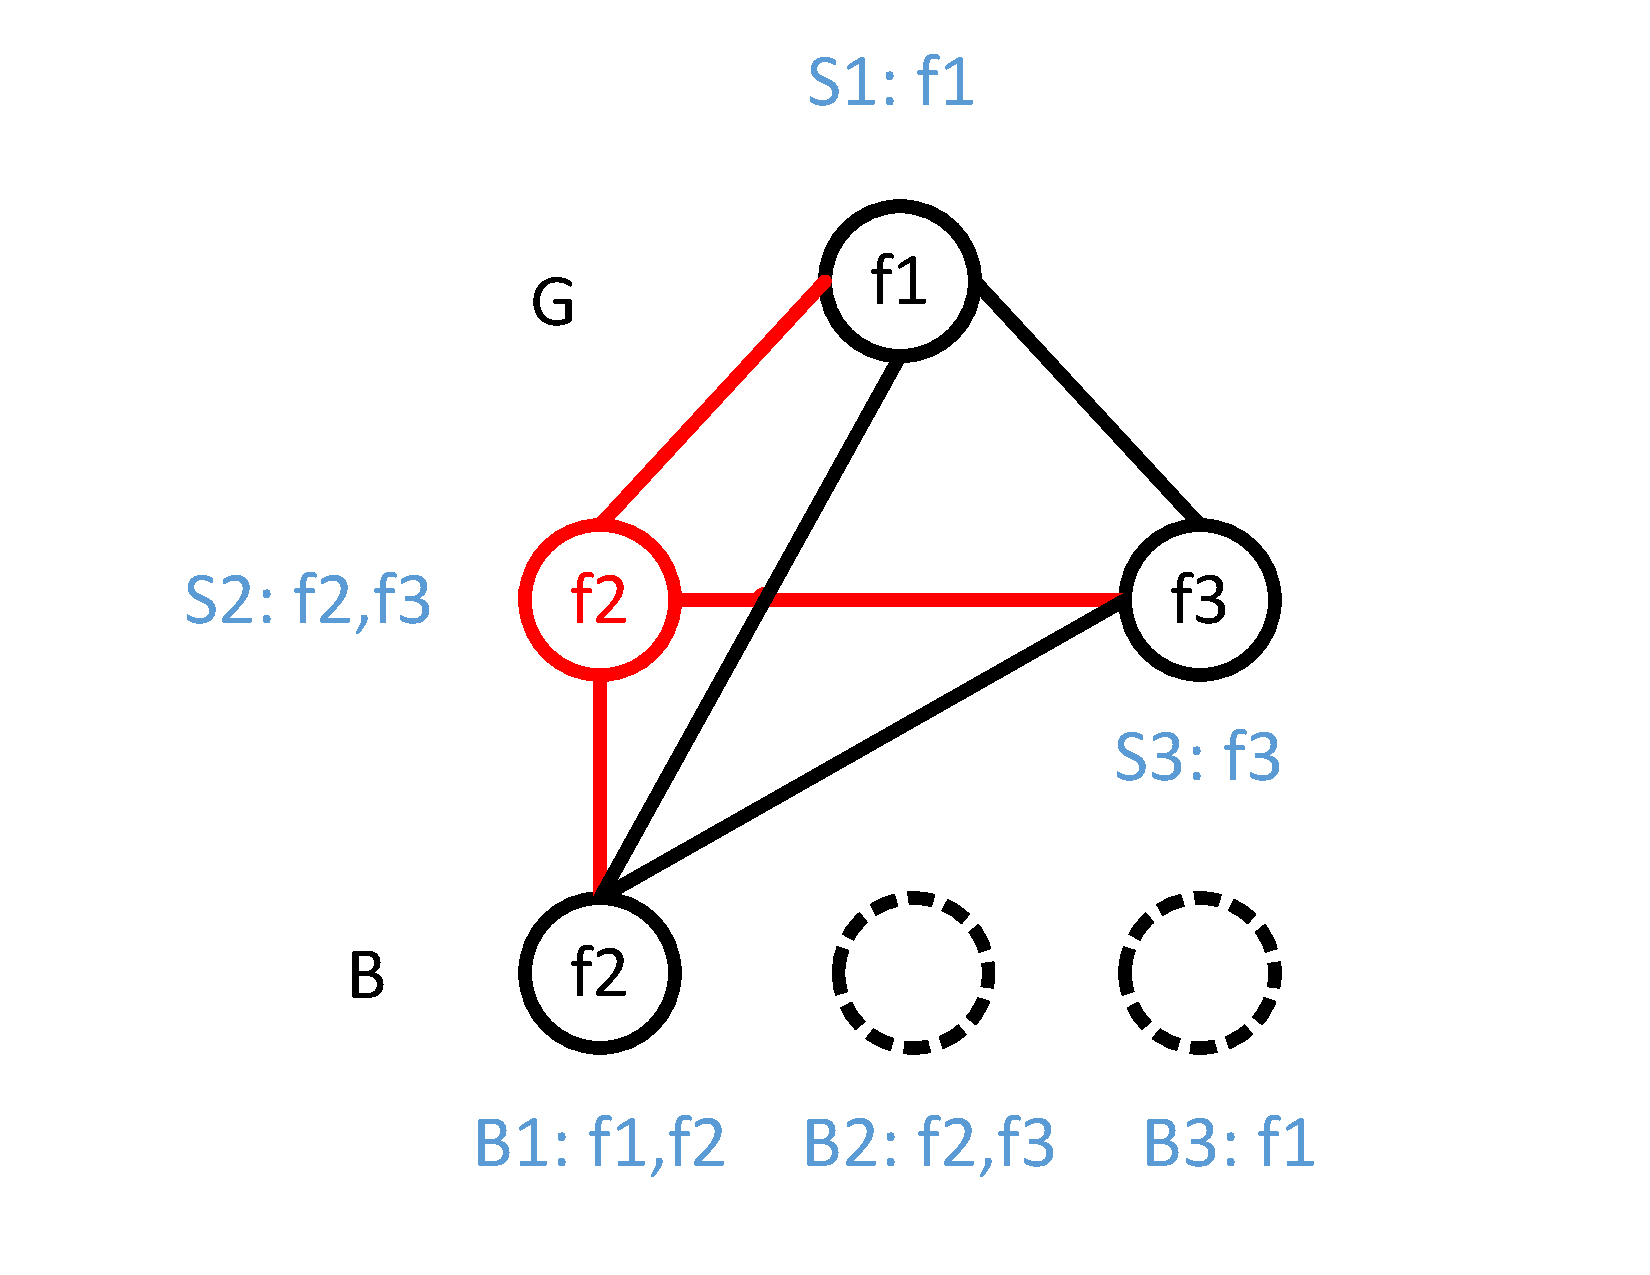
\includegraphics[width=1.5in]{Fig/SNFToptimal_n2Fail}\\
\caption{optimal $k$-FNFT($G(V,E,S),B(V,S)$) node $v_2$ fail, node $v_2$ transform to $b_1$}\label{fig:SNFToptimal_n2Fail}
\end{minipage}
\hfill
\begin{minipage}[t]{0.3\linewidth}
\centering
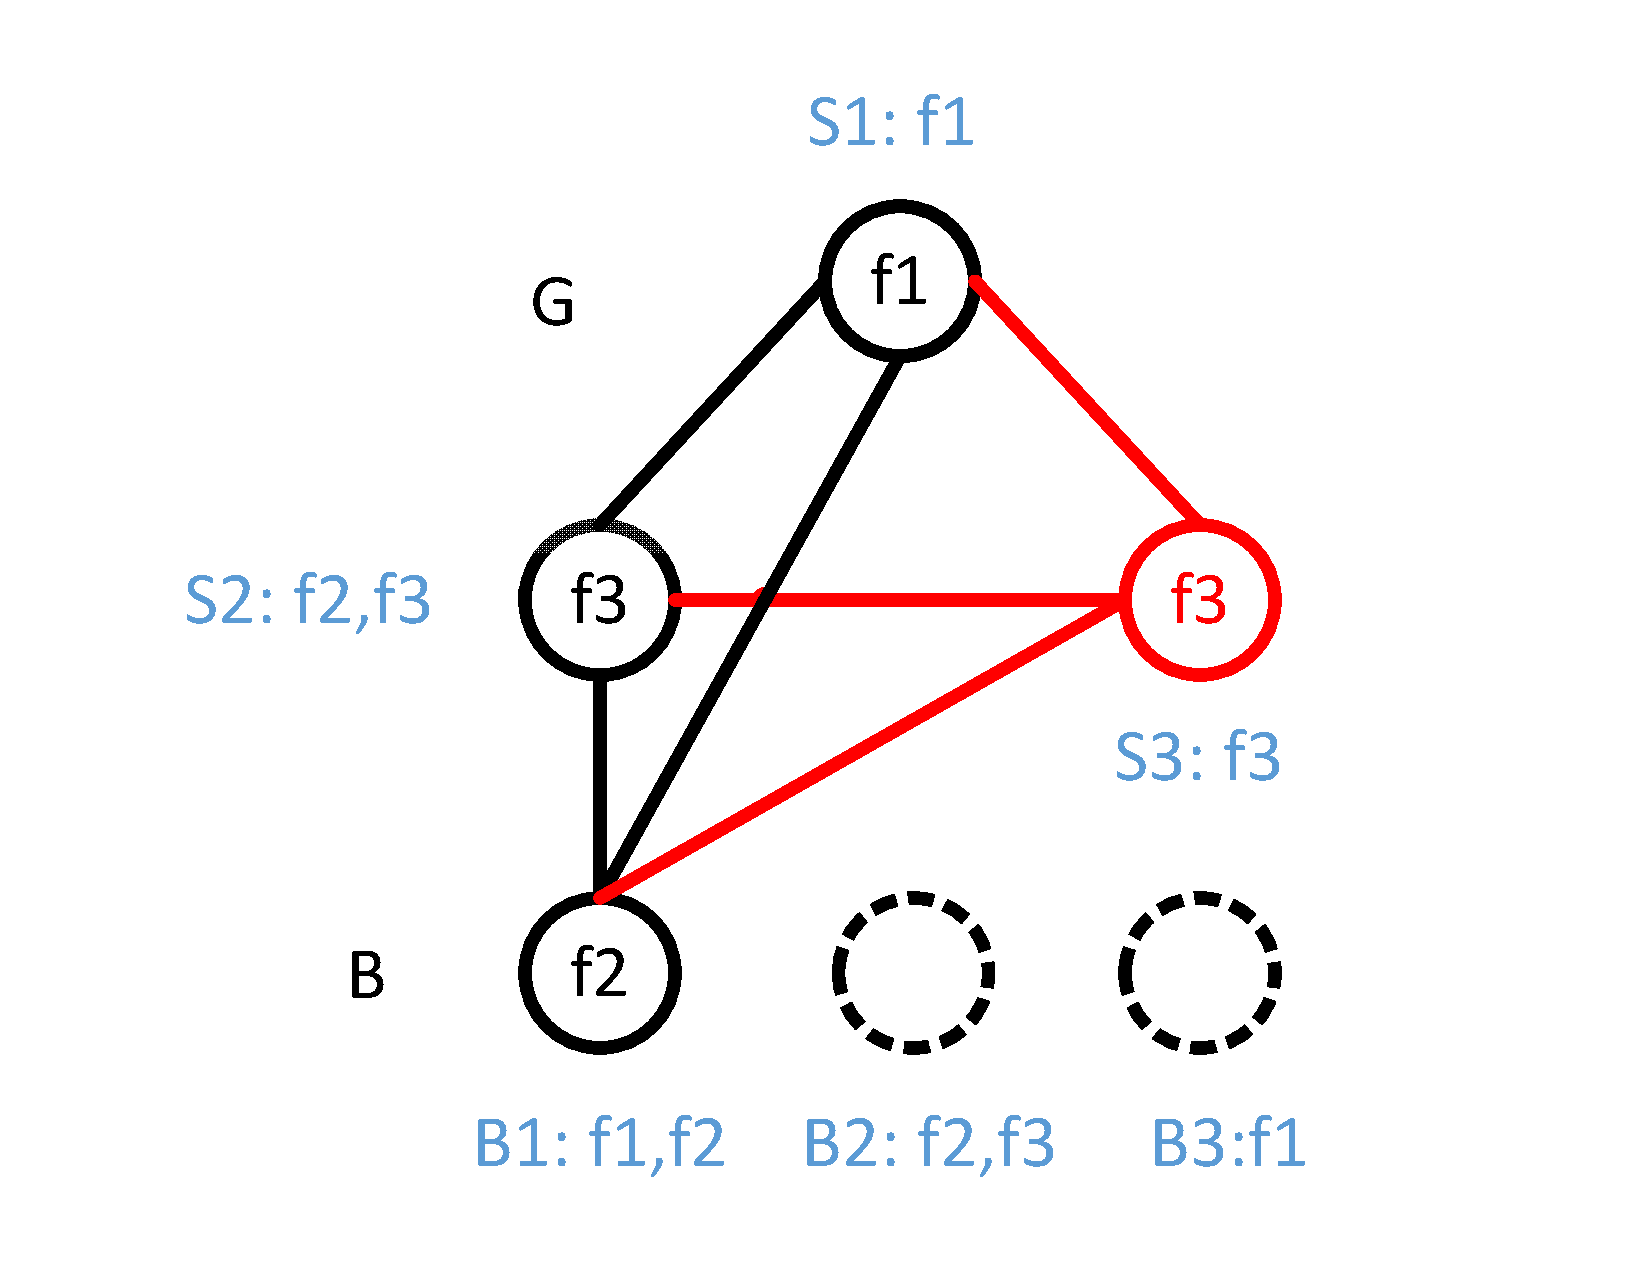
\includegraphics[width=1.5in]{Fig/SNFToptimal_n3Fail}\\
\caption{optimal $k$-FNFT($G(V,E,S),B(V,S)$) node $v_3$ fail, node $v_2$ transform to $b_1$, node $v_3$ transform to $v_2$}\label{fig:SNFToptimal_n3Fail}
\end{minipage}
\end{figure*}

\subsection{Complexity of Function Node Fault tolerant}
\label{sec:Complexity}
This computation complexity of $k$-FNFT graph problem $k$-FNFT($G(V,E,S)$) is NP, whose proof is described as below. when just exist one function type in Graph $G$, the problem is degenerated into k-node fault-tolerant graph problem. when Graph $G$ just have one type of function, we must add k backup node and add some edges into graph $G$ to construct $k$-FNFT graph, meantime the degenerated problem is of equivalency to k-node fault-tolerant $k$-NFT graph problem , which had been proofed as NP problem\cite{harary1996node}.

when added node set is given and confirmed aforehand , $k$-FNFT($G(V,E,S)$) is subproblem of the problem $k$-FNFT($G(V,E,S),B(V,S)$). Therefore, according to  the  reducibility theorem\cite{cormen2009introduction} in computer complexity field, it is easy to conclude that problem $k$-FNFT($G(V,E,S),B(V,S)$) is NP problem also.

The inter-inclusion relationship of the three problem is $k$-FNFT($G(V,E)$)$\subset$$k$-FNFT($G(V,E,S)$)$\subset$$k$-FNFT($G(V,E,S),B(V,S)$).

%Suppose topological structure of graph $G$ is path $P$, k-FNFT($P(V,E,S),B(V,S)$) is NP, the proof is below, exist one node $v_i(v_i\in V)$ and we add backup nodes and some edges to protect the node $v_i$, the former graph $P$ firstly is changed into $P+n$, nevertheless topological structure of $P+n$ may is not path, or be tree and non-tree graph. then protect other nodes of $V$ except node $v_i$, the problem become $(k-1)$-NFT problem.



However, this poses a limitation since the result only guarantees graph isomorphism and not equality without considering constraints of computation and communication. In other words, there may be a need to physically swap remaining VMs while recovering from some failure in order to return to the original infrastructure G. Recovery may then be delayed, or require more resources for such swapping operations.

%the computation complexity of k-FNFT($T(V,E,S),B(V,S)$) is similarly available.

%Edge fault tolerant problem is subgraph of node fault tolerant problem.




\subsection{Substrate Network}
Substrate network is referred as network functions virtualization infrastructure or physical network,  We model the Substrate network(SN) as an undirected attributed graph $G^S (V^S,E^S,F^S,C^S,B^S)$, where $V^S$ and $E^S$ is the set of substrate nodes and substrate links respectively, $F^S$ is the function type set on which substrate nodes can run. Each substrate node (link) is associated with the residual computing (communication) resource capacity. Each node $v_i$ has an available computational capacity of $c_i$. The node number of substrate nodes is $m$. Each undirected link $e_{ij}$ has an available bandwidth of $b_{ij}$. The number of function type is $p$. In Fig.\ref{fig:VNmapSN} (a),  substrate nodes set $V^S$ is $\{S_1,S_2,S_3,S_4,S_5,S_6,S_7\}$, substrate nodes's unction type set $F^S$ is $\{\{f_1\},\{f_2,f_3\},\{f_3\},\{f_4\},\{f_1,f_2\},\{f_1,f_4\},\{f_2,f_3\}\}$.

\subsection{Virtual Network Request Model}
A topological graph for a virtual network(VN) request is an undirected attributed labeled graph, denoted as $G^V (V^V,E^V,s^V,C^V,B^V)$, where $V^V$ corresponds to a node set, The node number of virtual nodes is $n$, $E^V$ denotes a set of bidirectional edges among the VN nodes and $f^V$ denotes a function type belonging the VN nodes. Each task node $v_i^V$ specifies the needed available computational resource $c_i^V$ ($c_i^V \in C^V$), and each edge $e_{ij}$ specifies the requested amount of communication (bandwidth) resource $b_{ij}^V$ ($b_{ij}^V \in B^V$) as shown in Fig.\ref{fig:VNQ}.
\begin{figure}
\centering
% Requires \usepackage{graphicx}
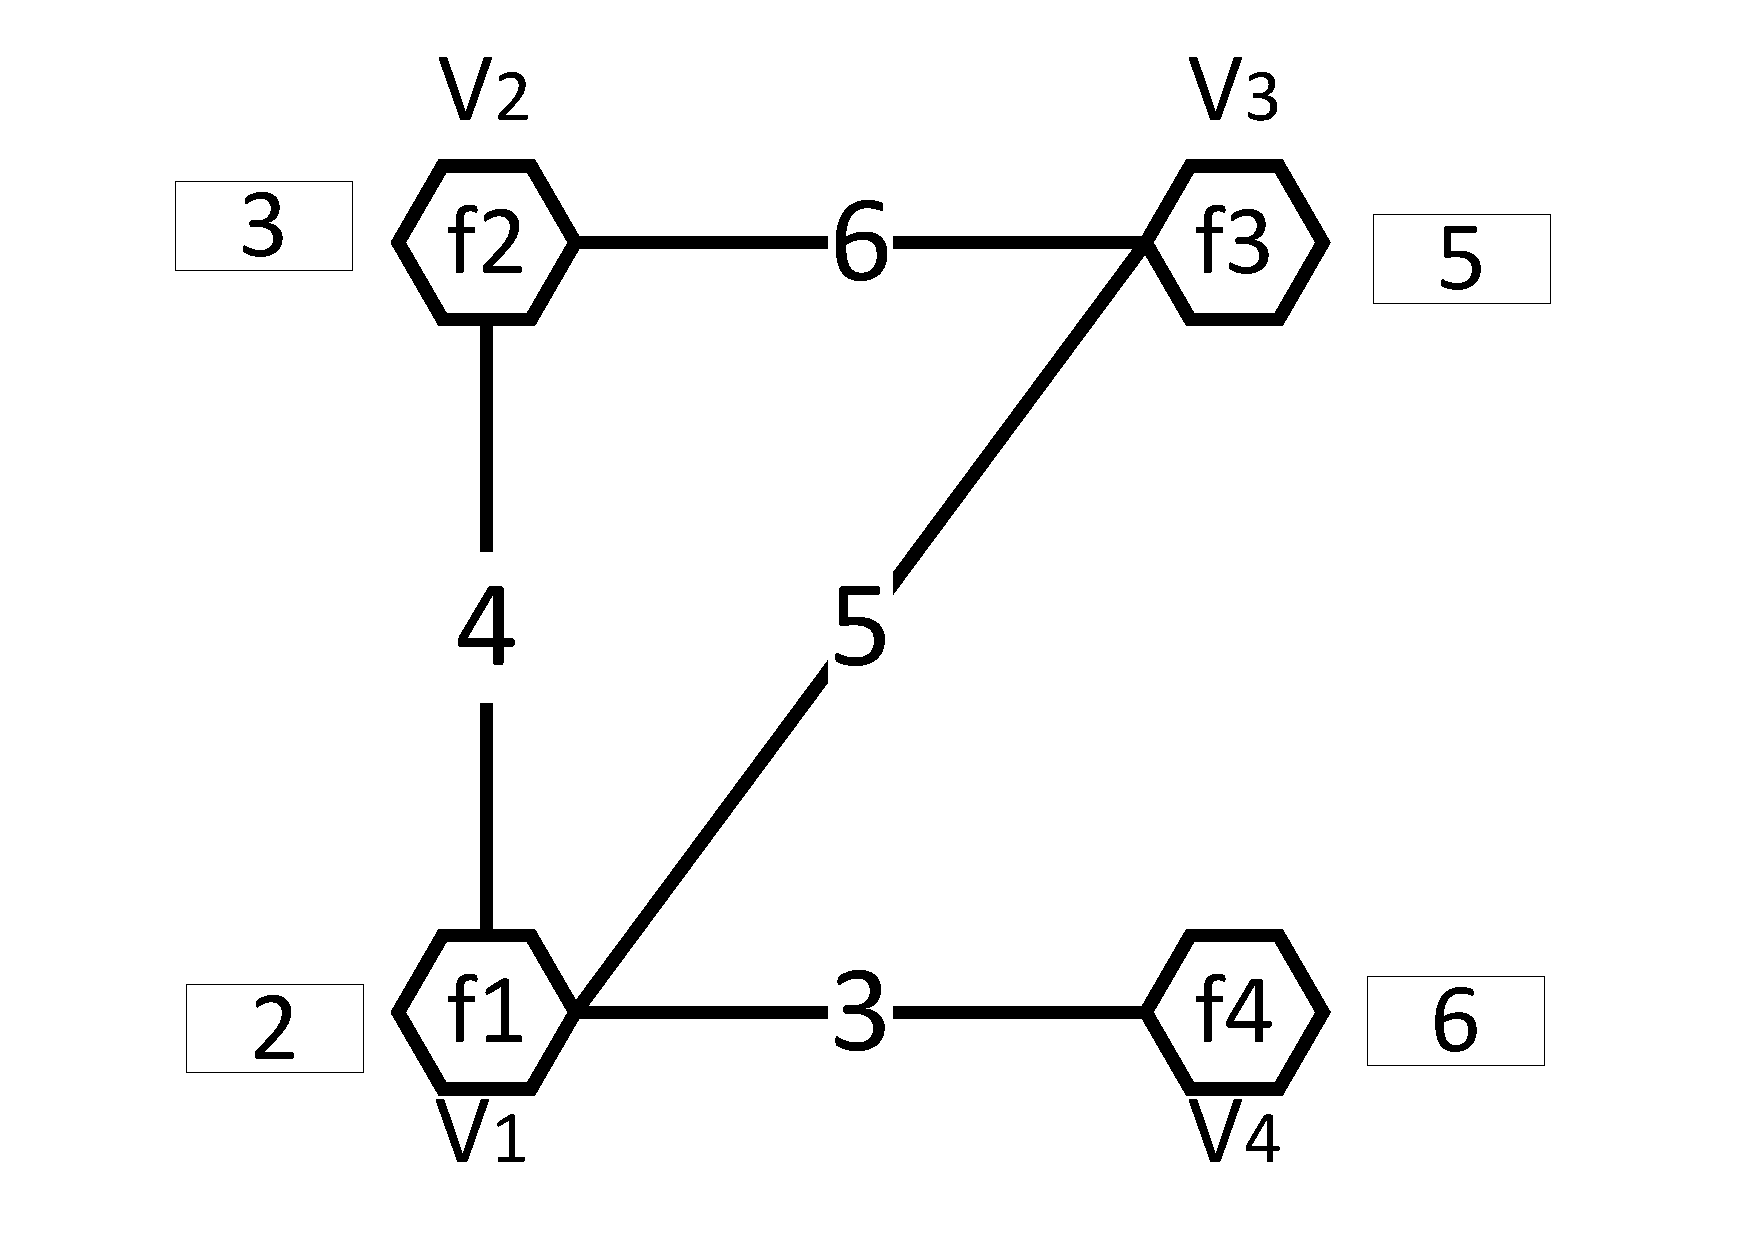
\includegraphics[width=2in]{Fig/VNQ}\\
\caption{Virtual Network Request $G^V (V^V,E^V,f^V,C^V,B^V)$, $V^V=\{v_1,v_2,v_3,v_4\}$,$E^V=\{e_{12},e_{23},e_{13},e_{14}\}$,$f^V=\{f_1,f_2,f_3,f_4\}$,$C^V=\{2,3,5,6\}$,$B^V=\{4,6,5,3\}$}\label{fig:VNQ}
\end{figure}

\subsection{Embedded Virtual Network}
\label{sec:embeddedVirtualNetwork}
There exist many approaches is modeled as the VN embedding (VNE) problem which attracts a broad interest recently\cite{fischer2013virtual}. VNE is extremely important in order to maximize the number of coexisting VNs and increase the utilization of substrate infrastructures. Most of the proposed approaches decompose the problem into two phases, the node embedding phase and the link embedding phase, to reduce the overall complexity of this problem. When a virtual network request has been inserted in to substrate network, augmented resource is attached into virtual network, embedded virtual network denote as $G^V (V^V,E^V,f^V,F^V,C^V,B^V,M^V)$ as shown in Fig.\ref{fig:eVN}. $F^V$ denote a set of function type set $F^V_i$($f^V_i\in F^V_i$) which corresponding to every VN nodes $v_i$. $C^V$ denote node's computational resource's capacity. $B^V$ denote edge's bandwidth resource's capacity. $M^V$ denote node's mapping relationship of virtual network embedding algorithm, $M_{i}=j$ represent that the i-th VN's node had been embedded at j-th substrate network node. Besides, with respect to the node embedding, we suppose a assumption that all virtual nodes of VN should be mapped on isolated physically substrate nodes.
\begin{figure}
\centering
% Requires \usepackage{graphicx}
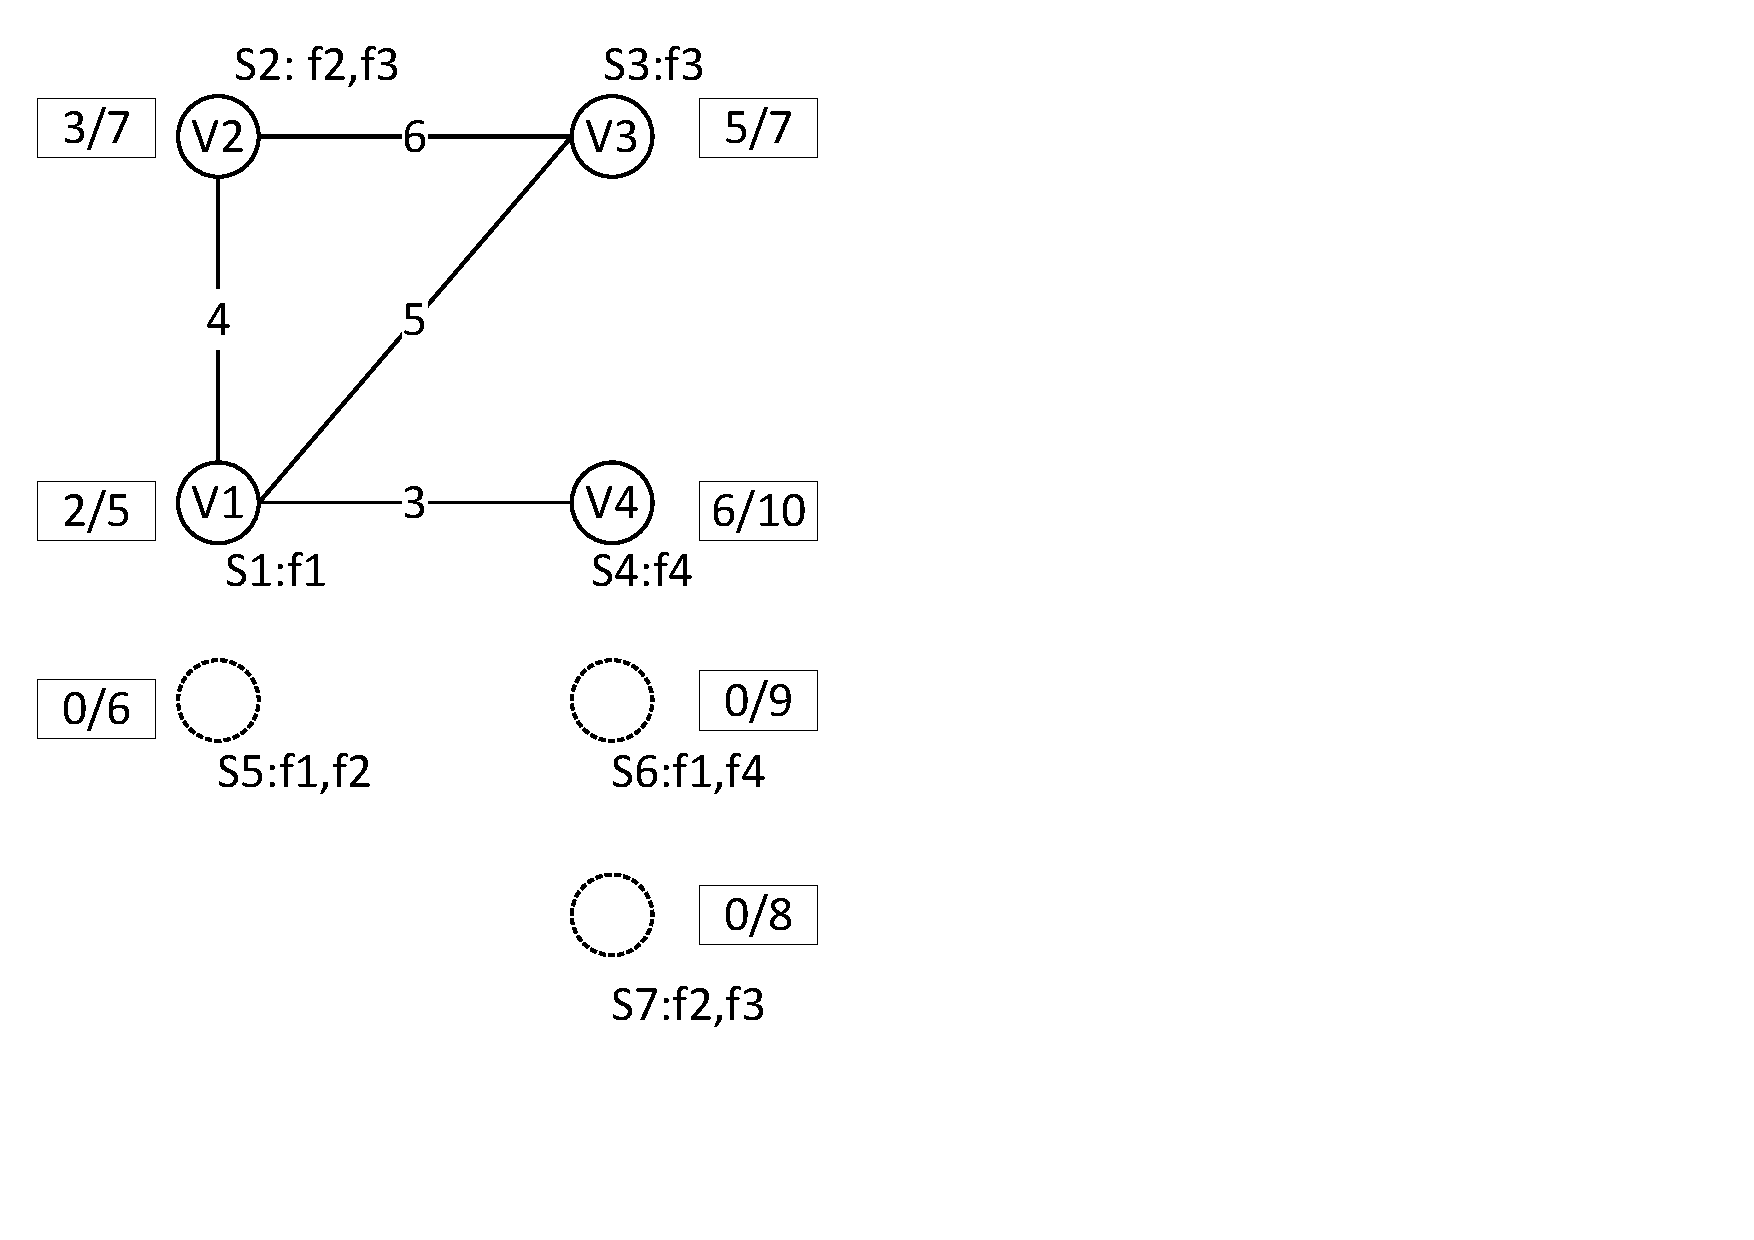
\includegraphics[width=2in]{Fig/eVN}\\
\caption{embedded Virtual Network $G^V (V^V,E^V,f^V,F^V,C^V,B^V,M^V_V)$,$V^V:\{s_1,s_2,s_3,s_4,s_5,s_6,s_7\}$,$E^V=\{e_{12},e_{23},e_{13},e_{14}\}$,$f^V:\{f_1,f_2,f_3,f_4\}$,
$F^V=\{\{f_1\},\{f_2,f_3\},\{f_3\},\{f_4\},\{f_1,f_2\},\{f_1,f_4\},\{f_2,f_3\}\}$,$C^V=\{5,7,7,10,6,9,8\}$,$B^V=\{4,6,5,3\}$,$M^V=\{s_1,s_2,s_3,s_4\}$}\label{fig:eVN}
\end{figure}

\subsection{Survivable}
%We define reliability as the probability that critical nodes of a VInf remain in operation, over all possible node failures. This is not to be confused with availability, which is defined as a ratio of uptime to the sum of uptime and downtime

Survivability is guaranteed on the set of critical nodes of a VN through redundant virtual nodes with backup nodes set $B(V,F)$, we suppose all virtual node as critical node in our algorithm. In Fig.\ref{fig:eVN}, node set $V$ of backup node $B(V,S)$ is $\{s_5,s_6,s_7\}$, function type set $F$ of node is $\{\{f_1,f_2\},\{f_1,f_2\},\{f_2,f_3\}\}$. A backup (redundant) node $b_i$ may not be able to assume full execution function of a failed critical node. Hence, the backup node may not have sufficient resources in terms of computation resource.


%\subsection{How many backups?}
%The number of backup nodes depend on the physical mapping, and the failure models of both the physical nodes and the virtual infrastructure.

%The problem is to  allocate least resources for a VN $G$, including redundancy such that a reliability guarantee of at least r is achieved.



\subsection{Survivable embedded Virtual Network Request}

In this subsection, we define the SeVN design problem as follows, for a given VN request with $|V|$ nodes, the VN had been already embedded in substrate network SN and every node running function $s_i(s_i\in S^V)$, protect the VN with some additional/augmented nodes and a set of appropriate links to connect these virtual nodes, and reserve sufficient computing and communication resources in these nodes and links to guarantee the restorability of VN request after a facility/substrate node failure.


There are different combinations of function type belonging all nodes of embedded virtual network, but there is only one type of function type running onto substrate node which corresponding one virtual node at one moment.

There exist many backup virtual nodes $B(V,S)$ which are abstracted from un-occupied substrate network's node. When one fault node $v_i$ appeared in virtual network request $G^V (V^V,E^V,s^V,C^V,B^V)$, Solving the survivable request of embedded virtual network is of approximately equivalence with asking 1-FNFT$(G,B)$ of graph $G$ and backup nodes set $B$ without computation and bandwidth's limitation.
%Generally speaking, survivable embedded virtual network's request is function node fault-tolerant of virtual network $G^V (V^V,E^V,s^V)$ with backup nodes set $B(V,S)$ without considering computation and bandwidth limitation.

Startup new node, connect link among nodes $V\cup B$, augment node computing or augment link bandwidth of existing link to construct $G^o$ as shown in Fig.\ref{fig:FD},\ref{fig:FI}, for which G is a subgraph of $G^o-R(R \subseteq V\cup B)$, $R$ is node set.We would connect some edges amongst nodes $V\cup B$ to construct FNFT graph of arbitrary graph $G$ as show Fig.\ref{fig:FD},\ref{fig:FI}, when only one node of VN failed, the topological graph of VN is also subgraph isomorphism of graph of SeVN, whose proof is describe as supposed in Sec\ref{sec:SubgraphIsomorphismProof}. %For example, when node v3 failed the node v2 run function 3 and backup node run function 2 so that the graph of VNR is subgraph isomorphism of SVN-v3 as shown in figure \ref{fig:optgraph_n1_fail},\ref{fig:optgraph_n2_fail},\ref{fig:optgraph_n3_fail}, the red edge and red node is disable.
%write the bandwith and computting resource between FI and FD.

\begin{figure}
\centering
\begin{minipage}[t]{0.5\linewidth}
\centering
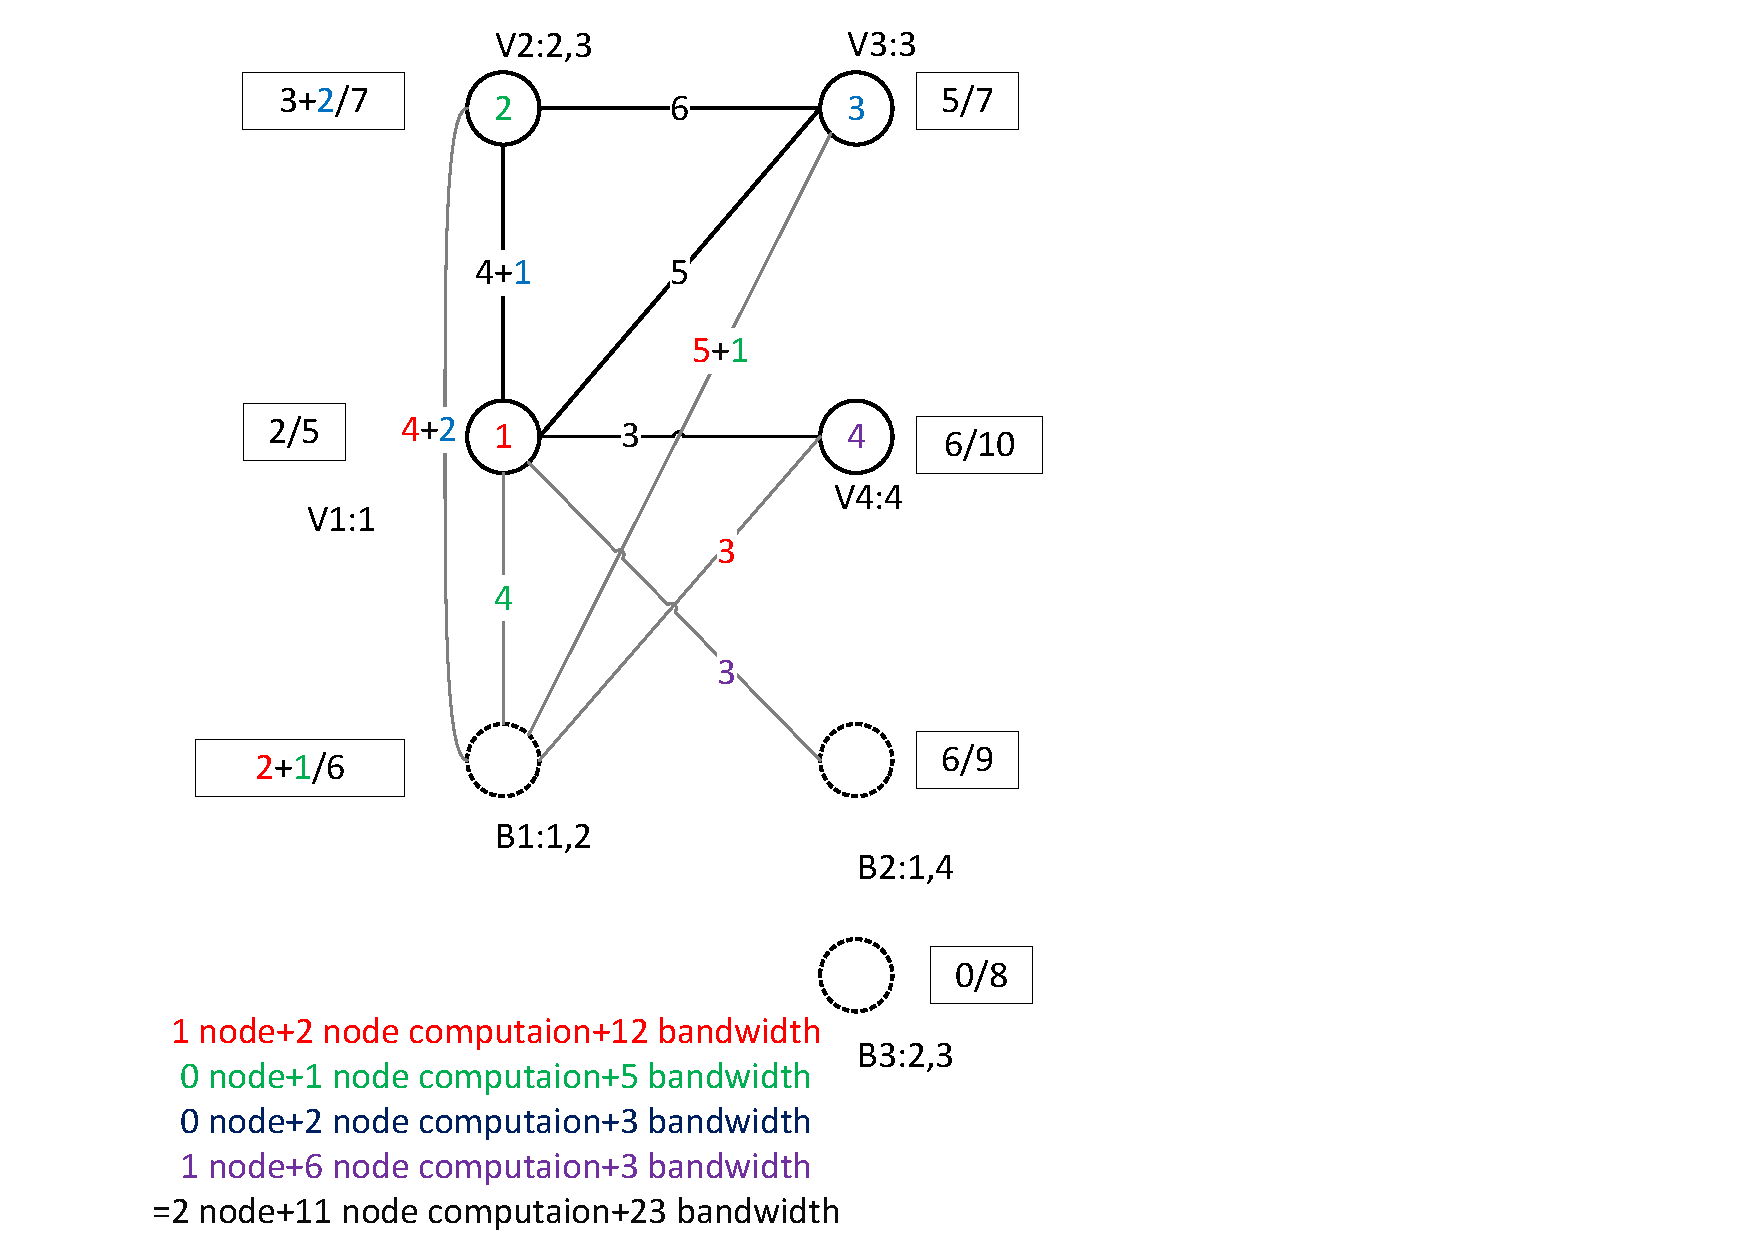
\includegraphics[width=2in]{Fig/FD}\\
\caption{ FD}\label{fig:FD}
\end{minipage}
\hfill
\begin{minipage}[t]{0.5\linewidth}
\centering
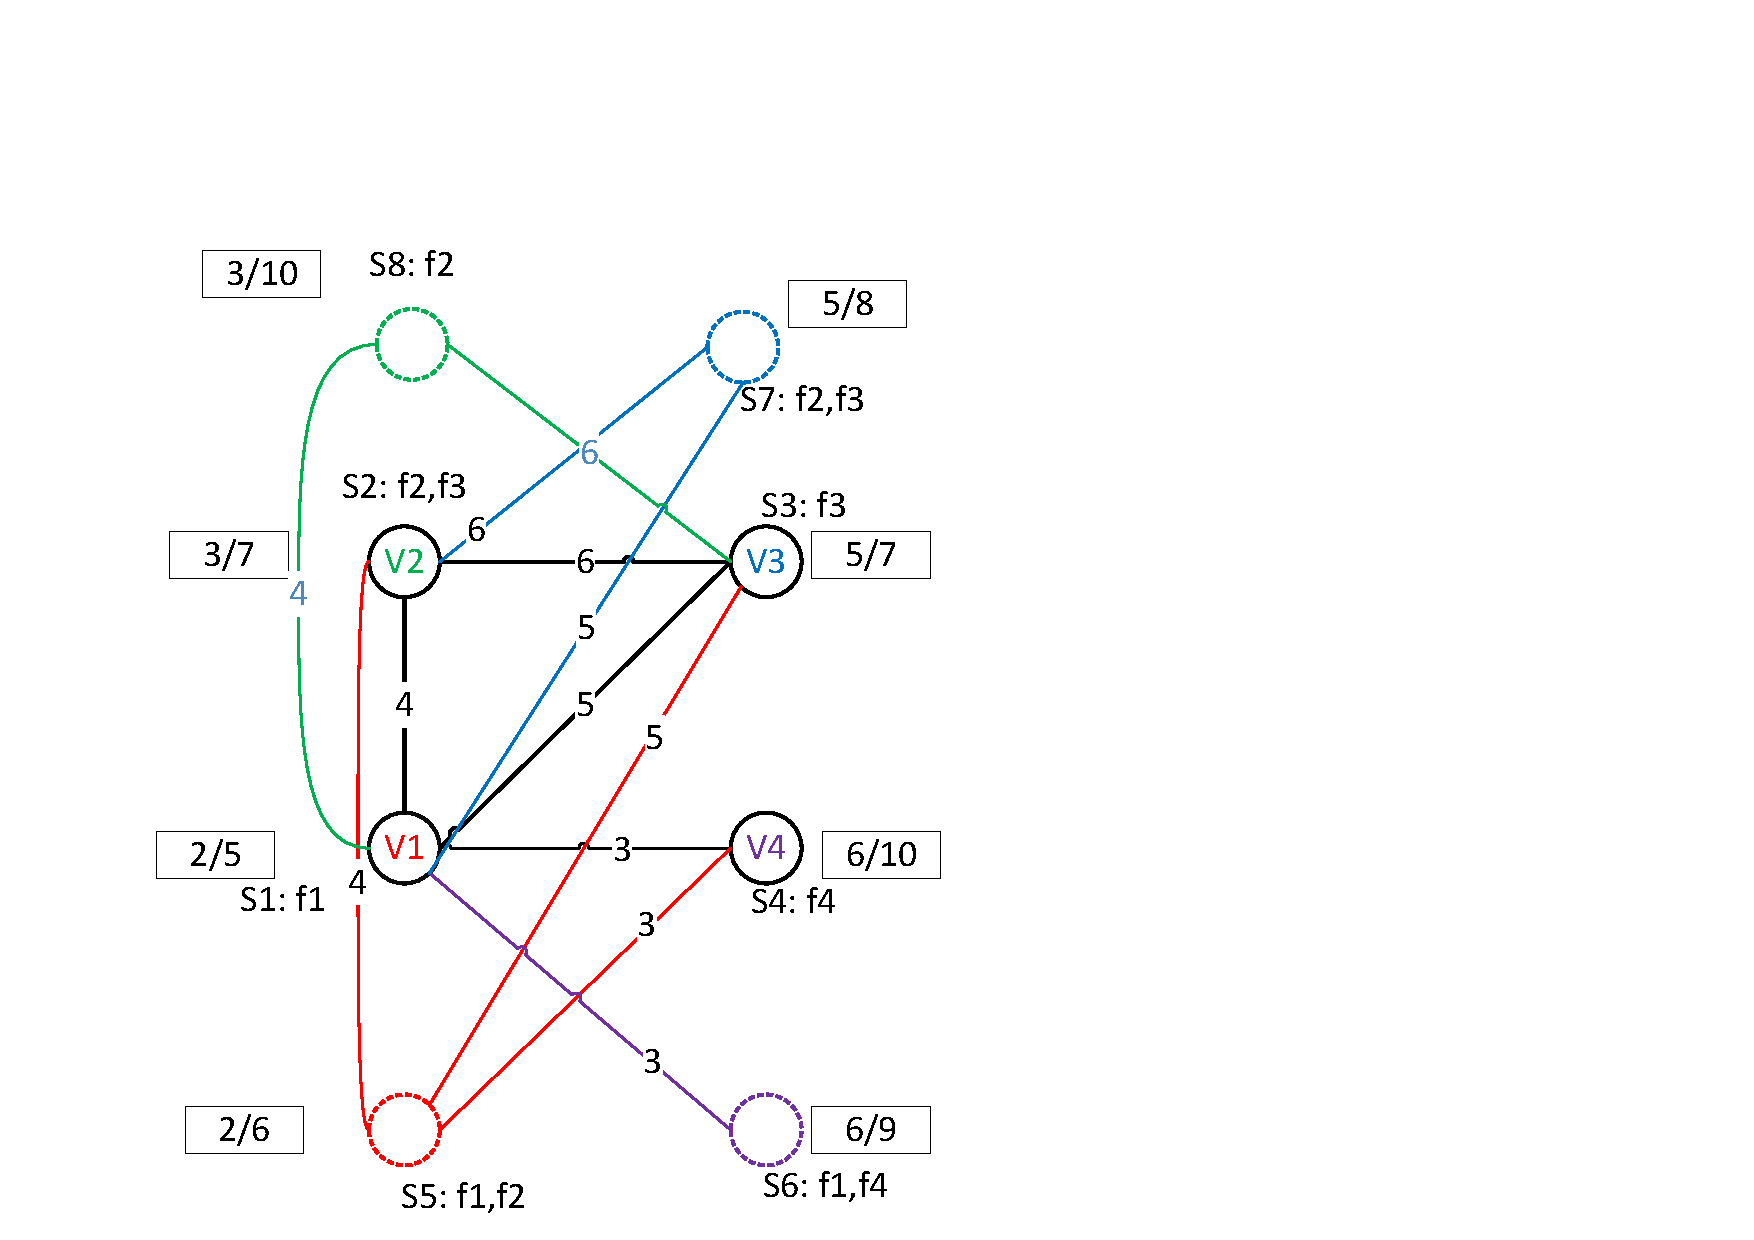
\includegraphics[width=2in]{Fig/FI}\\
\caption{FI}\label{fig:FI}
\end{minipage}
\end{figure}




